\section{Célula fotovoltaica}

A célula fotovoltaica é um dispositivo elétrico que converte a energia da luz diretamente em eletricidade pelo efeito fotovoltaico, que se trata de um fenômeno físico e químico [14]. É um dispositivo cujas características elétricas como corrente, tensão e resistência variam quando exposto a um tipo de luz.

Um dos exemplos mais visíveis e mundanos de uma célula fotovoltaica é o painel solar (conjunto de células solares ligadas entre si formando um circuito), comumente visto em residências, prédios e indústrias, conforme Figura \ref{fig:energia_solar_1}. Além de serem utilizados como produtores de energia elétrica, também são utilizados como fotodetectores (por exemplo, detectores de infravermelho), detectando luz ou outra radiação eletromagnética.

\begin{figure}[ht!]
	\centering
	\caption{Efeitos biológicos da Radiação Laser}
	\label{fig:energia_solar_1}
	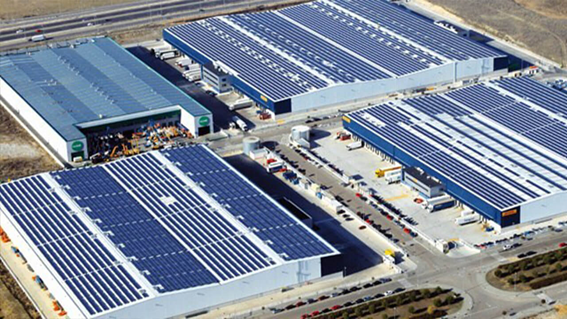
\includegraphics{energia_solar_1}[scale=1]
	\smallcaption{Fonte: \url{https://solarnog.com.br/energia-solar-para-o-setor-industrial/}. Acessado em: 22/05/2021.}
\end{figure}

\subsection{2.2.1	Evolução e história da célula fotovoltaica}

O surgimento da célula fotovoltaica se deu com o complemento de ações de dois indivíduos, um físico francês chamado Alexandre Edmond Becquerel e do inventor Chales Fritts. Alexandre foi a primeira pessoa a observar o efeito fotovoltaico, que é a base de funcionamento da célula fotovoltaica em 1839, porém somente em 1883 Chales Fritts criou a primeira célula fotovoltaica usando selênio, a eficiência da mesma não chegava a 1\%.

Com a chegada do século XX veio a explicação do efeito fotoelétrico por Albert Einstein, desenvolvimentos de processos de purificação e dopagem aplicadas a transistores, até que em 1954 foi anunciada a primeira célula fotovoltaica usando silício desenvolvida pelos pesquisadores dos laboratórios da Bell Calvin Fuller (químico), Gerald Pearson (físico) e Daryl Chapin (engenheiro) que podem ser vistos na Figura 6, a célula desenvolvida tinha apenas dois centímetros quadrados e atingia uma eficiência de até 6\%, gerando 5mW de potência elétrica [15].

\begin{figure}[ht!]
	\centering
	\caption{Calvin, Gerald e Daryl no laboratório da Bell}
	\label{fig:energia_solar_1}
	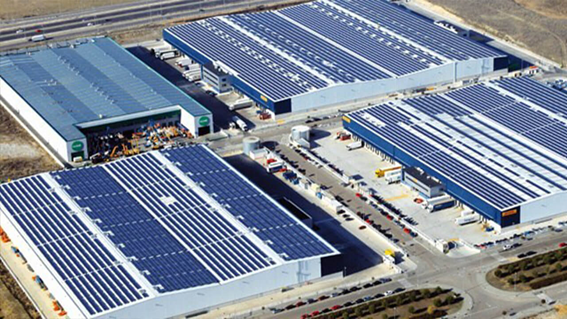
\includegraphics{energia_solar_1}[scale=1]
	\smallcaption{Fonte: \url{https://ambientes.ambientebrasil.com.br/energia/energia_solar/historico_das_celulas_fotovoltaicas_e_a_evolucao_da_utilizacao_de_energia_solar.html}.  Acessado em: 30/08/2021.}
\end{figure}

O primeiro painel instalado foi como fonte de alimentação de uma rede telefônica local em Americus, nos Estados Unidos em 1955. Em 1958 um painel de 1W foi anexado ao satélite Vanguard I para alimentar seu rádio durante a viagem pelo espaço. Com o passar das décadas foram desenvolvidos diferentes tipos de células solares, até que em 1999 a capacidade de energia instalada no mundo superou os 1000 megawatts, sendo que um ano depois foram constituídos sistemas fotovoltaicos conectados à rede elétrica na maioria dos países de Primeiro Mundo. Com o avanço da industrialização na China (2011), as fabricas de painéis e células se expandiram rapidamente, tornando os custos de fabricação cada vez menores, disseminando de vez a energia solar pelo mundo.

Até que em 2012 houve a regulamentação da RN 482 da Aneel no Brasil, que permitiu a qualquer consumidor gerar sua própria energia renovável conectada à rede de distribuição, com o acúmulo de créditos energéticos [16].

\subsection{Teoria}

A célula fotovoltaica funciona em várias etapas, inicialmente os fótons de luz atingem o painel e são absorvidos por materiais semicondutores como silício dopado. A placa de silício é montada com diversas camadas de material tipo P intercaladas com material tipo N, formando junções PN. A dopagem Tipo N consiste na dopagem do silício usando fósforo (mais comum) ou o arsênio. Ambos possuem 5 elétrons na camada de valência, como o silício contém 4 elétrons em sua camada de valência, a dopagem acontece de forma que um elétron fica de fora da ligação covalente com o silício por não ter a quem se ligar, tornando-se livre. A dopagem do tipo P consiste na dopagem do silício usando Boro. Este possui 3 elétrons na camada de valência, que quando feita a ligação covalente com os elétrons da camada de valência do silício sobra-se um elétron sem ligação proveniente do silício, desta forma, forma-se uma lacuna [17].

\begin{figure}[ht!]
	\centering
	\caption{Região de depleção}
	\label{fig:diodo}
	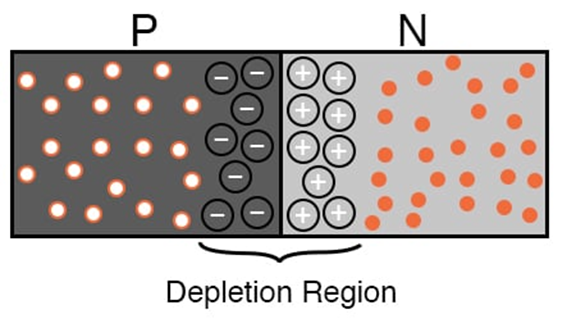
\includegraphics{diodo}[scale=1]
	\smallcaption{Fonte: \url{https://www.allaboutcircuits.com/video-tutorials/the-pn-junction-and-the-diode/}. Acessado em: 05/05/2021.}
\end{figure}

Nas proximidades das junções PN existem regiões de depleção (similares às observadas em diodos convencionais), que não existem portadores livres (elétrons e lacunas). Quando o feixe de luz incide na célula, os elétrons que estão nessas regiões de depleção, presos por ligações covalentes, ganham energia superando o \emph{energy gap}, que consiste na energia necessária para um átomo ``saltar'' da camada de valência para a camada de condução, gerando corrente elétrica. Ou seja, a incidência de fótons faz com que ligações covalentes se rompam e pares elétron-lacuna sejam formados.

\subsection{Composição de uma placa fotovoltaica}

A Figura \ref{pv_cell} mostra a estrutura de uma placa fotovoltaica, fica evidente a existência de diversos elementos, de forma a aumentar sua resistência e robustez [18].

\begin{figure}[ht!]
	\centering
	\caption{Funcionamento da célula fotovoltaica}
	\label{fig:pv_cell}
	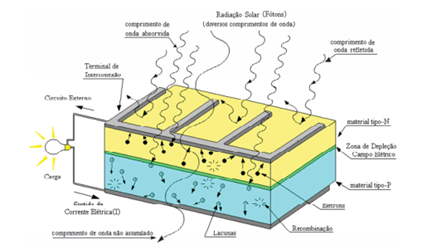
\includegraphics{pv_cell}[scale=1]
	\smallcaption{Fonte: GOETZE, Felipe. Projeto De Microgeração Fotovoltaica Residencial: Estudo De Caso.  2017. TCC (Graduação de Bacharel em Engenharia Elétrica) - Universidade Federal do Rio Grande do Sul, Porto Alegre, 2017. p. 22 – 24. Disponível em: \url{https://www.lume.ufrgs.br/handle/10183/169263}. Acesso em: 22 maio 2021.}
\end{figure}

A Figura 9 mostra a composição de uma placa fotovoltaica onde a célula é o agente produtor de energia, porém há outros componentes que fazem parte da estrutura de uma placa fotovoltaica. Dentro da placa, há um conjunto de células conectadas por uma faixa condutora ultrafina, tecida de cima para abaixo e conectando todas as células formando consequentemente um circuito. O conjunto de células conectadas ficam vedadas entre duas películas encapsulantes, colocadas sobre um fundo protetor chamado de \emph{backsheet}, onde as placas são conectadas em série por meio de uma caixa de junção. Por cima de uma das películas encapsulantes é posto um vidro temperado para proteção e, por fim, uma moldura de alumínio [19].

\begin{figure}[ht!]
	\centering
	\caption{Construção do painel solar}
	\label{fig:pv_cell_2}
	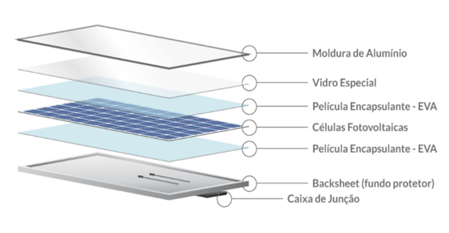
\includegraphics{pv_cell_2}[scale=1]
	\smallcaption{Fonte: CLEAN ENERGY REVIEWS. Most Efficient Solar Panels 2021. 2021. Disponível em: \url{https://www.cleanenergyreviews.info/blog/most-efficient-solar-panels}. Acesso em: 20 mai. 2021.}
\end{figure}

\subsection{Eficiência}

A eficiência de um painel fotovoltaico é medida através de quanto irradiação chega à placa é convertida em eletricidade. Devido aos recentes avanços da tecnologia fotovoltaica, a conversão média de um painel solar aumentou de 15\% para até 27\% [20]. Diversos fatores influenciam na eficiência de um painel fotovoltaico como posicionamento, orientação e condições climáticas.

Para determinar a eficiência de um painel é necessário testá-lo sob condições de teste padrões (CTP). As CTP especificam a temperatura a 25°C e um irradiação de 1000\mbox{$W/m^2$}. Isso é equivalente a um dia ensolarado com uma luz incidente atingindo uma superfície inclinada a 37° voltada para o sol.

Existem diversos tipos de painel fotovoltaicos. Os tipos mais comuns são: 

\begin{itemize}
	\item Painéis Monocristalinos
	\item Painéis Policristalinos
	\item Painéis \emph{Thin-film}
\end{itemize}

É importante entender que a eficiência de uma célula individual não equivale a eficiência de um painel (conjunto de células) como um sistema. Enquanto a eficiência de um painel é em torno de 15-27\%, a eficiência de uma célula solar pode atingir até 42\% em alguns casos.

Os painéis monocristalinos, são fabricados do mais puro silício. Um cristal desse tipo de silício é feito através de um processo complexo para produzir um logo cilindro de silício chamado de tarugo. O tarugo é então cortado em wafers que farão parte do painel. Os painéis monocristalinos são conhecidos por entregar uma eficiência maior em CTP que outros 2 tipos mais comuns de painéis.Um painel atual de silício monocristalino pode entregar uma eficiência em torno de 22-27\%. Os painéis monocristalinos são reconhecidos pelas suas bordas redondas e cor escura.

Os painéis policristalinos são levemente menos eficientes que aqueles feitos de silício monocristalino. Isso é devido à natureza da produção. O silício não é feito como uma única célula, mas como um bloco de cristais. Estes blocos são então cortados em \emph{wafers} para produzirem os painéis. A eficiência padrão de um painel policristalino está entre 15-22\%. Os painéis policristalinos são reconhecidos pelo seu corte quadrado e cor azulada.
   
Painéis \emph{Thin film} são feitos cobrindo um substrato de vidro, plástico ou metal com um ao mais finas camadas de material fotovoltaico. Estes painéis são flexíveis e leves. É conhecido que os painéis \emph{thin film} degradam mais rápido que os monos e policristalinos. A eficiência padrão é de em torno de 15-22\% [21].